\documentclass[11pt, a4paper]{report} 
\usepackage[T1]{fontenc}
\usepackage{geometry}
\usepackage[onehalfspacing]{setspace}
\usepackage{titlesec}
\usepackage{graphicx}
\usepackage{float}
\usepackage{amsmath}
\usepackage{chngcntr}
\usepackage[numbers]{natbib}
\bibliographystyle{plain}
\parindent0cm

\title{Transcriptome Analysis of Cladophialophora immunda}
\author{Christina Kustor}
\date{August,2015}


\begin{document}
	\pagenumbering{gobble}
\newpage
\begin{center}

\includegraphics{boku_logo}\\
\smallskip
\large {Universit\"at f\"ur Bodenkultur Wien\\
University of Natural Resources and Life Sciences Vienna\\
\bigskip \bigskip \bigskip
\textbf{Department of Biotechnology}\\
Extremophile Center}\\
\bigskip \bigskip
\LARGE\textbf{Transcriptome Analysis of\\
\textit{Cladophialophora immunda}}\\
\bigskip
\large {Master Thesis\\
\bigskip \bigskip \bigskip
submitted by\\
Christina Kustor, BSc.\\
Vienna, 2015\\
\bigskip \bigskip \bigskip \bigskip
Supervisor: Katja Sterflinger-Gleixner, Assoc. Prof. Dr.\\
Co-Supervisor: Hakim Tafer, Dr.\\}
\end{center}

\newpage
Acknowledgement
\newpage
\pagenumbering{arabic}
\large \textbf{Abstract}\\
... \\
Keywords: 
\newpage
\large \textbf{Zusammenfassung}\\
...\\
Stichw\"orter: 
\newpage
\tableofcontents
\newpage
\setcounter{chapter}{1}
\counterwithout{figure}{chapter}
\setcounter{figure}{0}

\chapter*{Background} 
\addcontentsline{toc}{chapter}{Background}
\section{Black yeasts' reaction on different environmental conditions} 
Black yeasts differ from the most fungis because they can grow in extreme environments and are resistant against high levels of stresses like Ozon, UV and radioactivity. \cite{Gostincar2010} 
....


The aim of the thesis was to determine the transcriptomes of \textit{Cladophilaphora immunda}  and to understand which genes are transcribed under different conditions. The transcriptome data were obtained with RNA-seq performed by Ion Torrent technology coupled with the Ion Proton sequencer (Life Technologies, Carlsbad, CA) \cite{Blasi2015} and the analysis were realised with bioinfromatics methods.  
A workflow system for genome annotation with RNA-seq data was developed and followed by performing statistics to obtain a list of genes and their expression level differences between two groups. Furthermore functional annotation and additonal enrichment analysis were performed.

\newpage
\section{Cladophialophora immunda}
The black yeast \textit{Cladophialophora immunda} is known for the capability to grow on polyaromatic hydrocarbons and moreover for the ability to degrate hydrocarbons. \cite{Sterflinger2015} \textit{Cladophialophora immunda} was isolated from a gasoline station, in a hydrocarbon rich environment. Previous studies with bioredimiation spotted that \textit{Cladophialophora immunda} is able to grow on toluen and also can degrade toluen. \cite{Prenafeta-Boldu2001} \cite{Poyntner2014}


For the experimental conditions, the cultivation of \textit{Cladophilaphora immunda} in glucose and toluen was chosen. 


\newpage
\section{Transcriptome Analysis using RNA-seq}
The powerful technology RNA-seq and the analysis of transcriptomes, to know which gene is expressed, became an important method in science. Transcriptome analysis enablies the understanding of how sets of genes work together to form metabolic, regulatory and signaling pathways within a cell. \cite{Xiong2006} A distinction of RNA-seq from earlier methods, such as microarrays, is the high throughput of current RNA-seq platforms, the sensitivity afforded by newer technologies and the ability to discover novel transcripts, gene models and noncoding RNA species. \cite{Korpelainen2014} 

\bigskip
The work in the laboratory included the extraction of total RNA with FastRNA PRO RED KIT (MP Biomedicals, Santa Ana, CA), furthermore the isolation by means of Dynabeads mRNA DIRECT Micro Kit (Ambion by Life Technologies, Carlsbad, CA), transcriptome library preparation based on the Ion Total RNA-Seq Kit v2 (Life Technologies, Carlsbad, CA) and the key part, the RNA-Seq, implemented by Ion Torrent technology coupled with the Ion Proton sequencer (Life Technologies, Carlsbad, CA). \cite{Blasi2015}
\newpage
\section{Bioinformatics methods}
The increasing use of next-generation sequencing methods is related to a large amount of produced data, which has to be analysed and interpreted. Therefore bioinformatics methods are a necessary step in analysing transcriptomes. As RNA-seq is an active field of research producing new approaches and tools at a rapid pace, many alternative programs exist for each analysis step. \cite{Korpelainen2014}

\subsection{Workflow Systems}
The data analysing steps were performed by different programs and tools, which may need specific data formats and external files. The multiple steps can be handled through scripting a reusable pipeline with defined inputs, output and parameter for each step. 

The software Snakemake was used to evolve the pipelines for genome annotation, functional annotation and enrichment analysis. Snakemake is based in Python language and can be used on a single core workingstation as well as on a cluster without modifying the workflow. 
Snakemake's option "--dag" creates the directed acyclic graph (DAG) of executed jobs. \cite{Koster2012}  
\newline
In figure \ref{fig:DAG} exemplified the DAG of the enduced Snakemake file. Jobs (i.e. the execution of a rule) are depicted as nodes, a directed edge between two jobs means that the rule underlying the second job needs the output of the job executed before as an input file. A path represents a sequence of jobs that have to be executed serially.
\begin{figure}[H]
	\centering	
	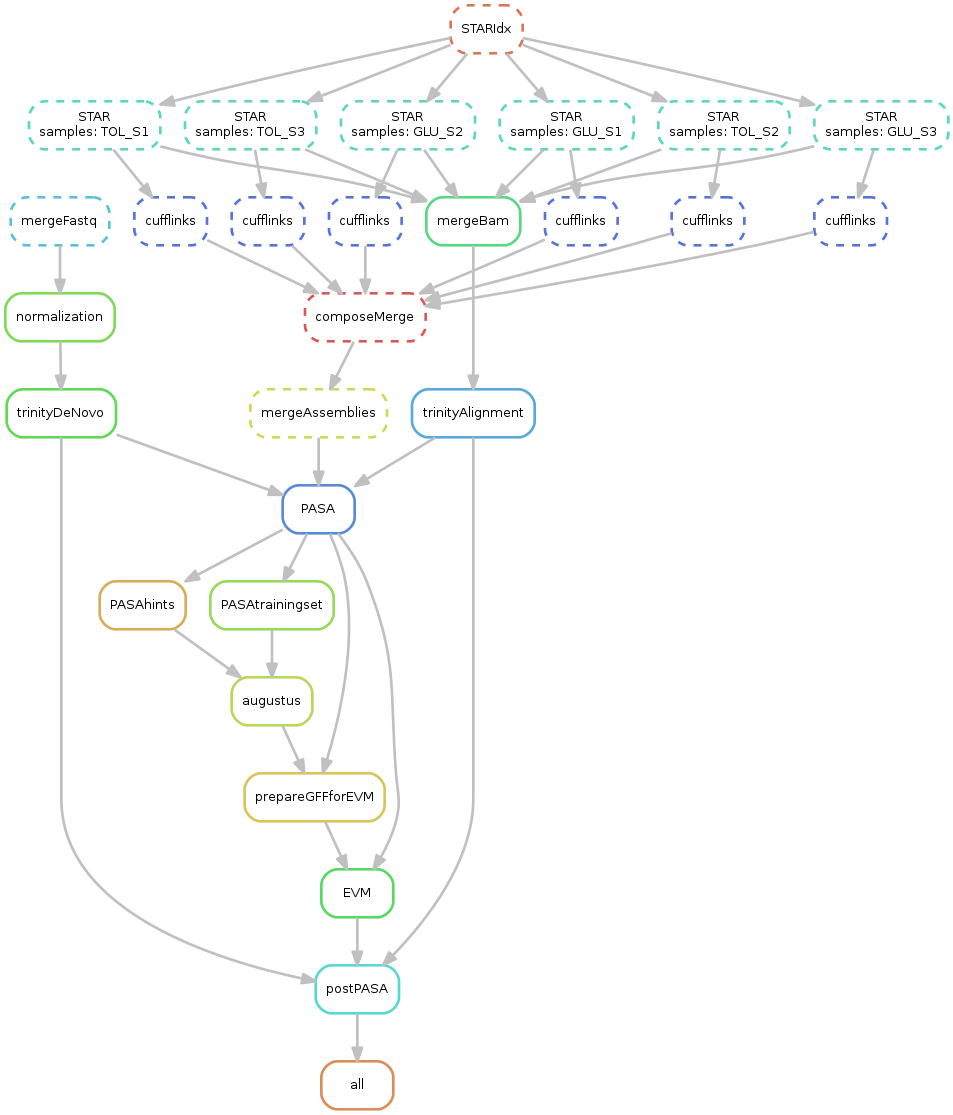
\includegraphics[width=400pt]{DAG.png}
	\caption[Directed acyclic graph (DAG)]
	{Directed acyclic graph (DAG) of a Snakemakefile}
	\label{fig:DAG}
\end{figure}
\newpage
\subsection{Algorithms}
\subsubsection{Maximum Mappable Length}\label{MML}
The algortihm Maximum Mappable Length (\textit{MML}) was developed to align reads to the genome. 
The idea of \textit{MML} approach is to search a Maximum Mappable Prefix (\textit{MMP}). Given a read sequence \textit{R}, read location \textit{i} and a reference genome sequence \textit{G}, the \textit{MMP(R,i,G)} is definde as the longest substring  
\[
		 [R_{i} , R_{i+1} , ... , R_{i+MML-I} ]
\]
which matches exactly one or more substrings of G, where \textit{MML} is the maximum mappable length. 
Starting from the first base of the read the algorithm finds the \textit{MMP}. If \textit{MMP} can not be mapped contigously to the genome, because of an splice junction, this first seed will be mapped to a donor splice site. The \textit{MMP} search is repeated for the unmapped portion of the read, which will be mapped to an aceptor splice site.
The difference to other algorithmn is to align the non-contigous sequences directly to the reference genome, which accelerated the process to map. \cite{Dobin2013}
\subsubsection{Expressed Sequence Tag}\label{EST}
Expressed Sequence Tag (EST) was evolved in early days of genome assembly. First the same assemblers where used for transcriptomes, but there a fundamental differences between genome assembly and transcriptome assembly. In the genome assembly the ideal output is a linear sequence representing each genomic region, whereas in the transcriptome assembly the gene is most naturally described as a graph.  \cite{Korpelainen2014}





\subsubsection{de Bruijn Graph}\label{Graph}
Each node of a de Bruijn Graph is associated with a (k -1)-mer. Two nodes A and B are connencted if there is a k-mer whose prefix is the (k -1)-mer of the node A and the suffix is (k - 1)-mer of the node B. The k-mers create edges in the Buijn graph. \cite{Korpelainen2014}

\newpage
\setcounter{chapter}{2}\setcounter{section}{0}
\chapter*{Methods}
\addcontentsline{toc}{chapter}{Methods}
Before implementing the workflow system a comparison of publications, different programs and tools were done. The choice of a suitable program depended on the kind of analysis and the amount of time is required. Another important issue was the option available of the used program. 

Six samples of reads were downloaded from the sequencer, three of them were the transcriptomes of \textit{Cladophialophora immunda} cultivated with glucose and the other three with toluen.
In the beginning the reads' origin was identified by aligning them to a reference genome with STAR. Mapped reads were used to perform transcript assembly with the softwares Cufflinks and Trinity Genome Guided. Trinity also was employed for mapping-free transcript assembly. With the produced assemblies from Cufflinks and Trinity, the Program to Assembly Spliced Alignments (PASA) performed the spliced alignment mapping. PASA assemblies were utilized to create hints for the location of introns and exons. Those hints were ingrated in a hintbased run of Augustus. Evidence Modeler (EVM) was used to combine weighted predictions. The last step was a annotation update implemented by PASA, where the output of EVM compared to PASA alignment assemblies and generated a updated gene set. \cite{Haas2011} \cite{Steijger2013} \cite{Linde2015}

Figure \ref{fig:pipeline} shows the draft of the entire workflow system for genome annotation with transcriptomic data. The inputs are the transcriptomes from RNA-Seq in bam-format, the genome in fasta-format and the de novo annotation without RNA-Seq data in gff3-format. After runs of the different steps the output is an annotation file in gff3-format.
\begin{figure}[H]
\centering	
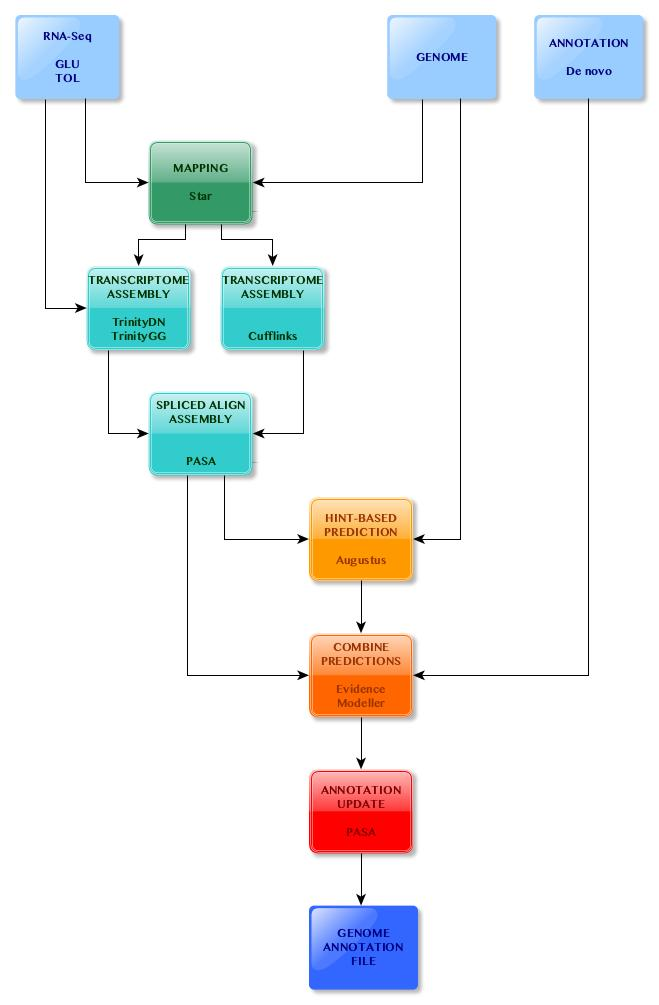
\includegraphics[width=360pt]{pipeline}
\caption[Genome Annotation Workflow]
{Genome annotation workflow system}
\label{fig:pipeline}
\end{figure}

\section{Alignment}
The first step to understanding a genome structure is through genome mapping, which is a process of identifying relative locations of genes on a chromosome. When a read is mapped to reference genome, a sequence alignment is created. \cite{Xiong2006} The input files in this case were the preprocessed reads and in addition the reference sequence. 
\subsection*{STAR}
Mapping is computationally intensive, that is why the program STAR was chosen. STAR (Spliced Transcripts Alignment to a Reference) is a spliced alignment program which runs very fast. The benefits of STAR are largely based on the "maximum mappable length" approach described in \ref{MML}. STAR splits a read and find the best portion that can be mapped for each piece. Then it maps the remaining portion, which can be far away in the case of a splice junction. The maximum mappable seed search looks for exact matches and uses the genome in the form of uncompressed suffix arrays. The second step of STAR stitches the seeds together within a given genomic window and allows mismatches, indels and splice junctions. The seeds from read pairs are handled concurrently at this step in order to increas sensitivity. \cite{Dobin2013} \cite{Korpelainen2014} 

The execution of STAR allocated in two parts, building a reference index and mapping. Before running STAR mapping it was obtained a reference index of the genome. Mapping of the reads was executed without the soft clip aligning at reference ends. The mapped reads needed to be sorted by Samtools. 

\section{Transcriptome Assembly}
The goal of RNA-seq assembly is to reconstruct full-length tanscripts based on sequenced reads. 
Transcript assembly answers the questions about exon regions and splice site. Several transcripts may overlap at different regions or there may be multiple copies of the same transcript.

There are two ways of performing transcriptome assembly. If there is a reference genome, it can be realised to guide the assembly, where the assembly task consits of solving which mapped reads correspond to which transcript. The second possibilty is to perform de novo assembly. \cite{Korpelainen2014} 
\subsection*{Cufflinks}
The software packages Cufflinks can be used for \textit{ab intio} reconstruction. The program within in this packages Cufflinks assembles transcriptomes from RNA-Seq data. 

Cufflinks reports the smallest possible set of isoforms. 


The program Cuffmerge was used to merge the multiple assembled transcriptomes into a master transcriptome. 
\cite{Trapnell2010}


The rule Cufflinks was implemented with the following option and values, the maximum intron length(2000) and the minimum intron length (30), the maximum number of fragment a locus may have before skipped(10000) and the library-type ff-firststrand.



\subsection*{Trinity}


\cite{Grabherr2013}

Trinity genome guided

Trinity de novo

\subsection*{PASA}
\section{Gene Prediction}
\subsection*{Augustus}
Augustus is an \textit{ab intio} gene predictor, where only a genomic sequence is needed as input information. In addition it is possible to use hints of various information. For the prediction Augustus combines genomic sequence alignments and alignments of expressed sequenced tags (EST), described in \ref{EST}. The model underlying the program is generalized hidden Markov model (GHMM). HMMs and GHMMs for gene prediction define a probabilty for each pair ($\mathrm{\varphi}$,s) of a sequence s and a gene structure $\mathrm{\varphi}$. Before starting the program Augustus it is necessary to train the model. \cite{Stanke2006} 

The trainingset was created from PASA assemblies by executed the program "pasa\_asmbls\_to\_training\_set.dbi" included in PASA package. For the additional file of hints the location of introns were filtered from PASA assemblies. Subsequently Augustus was started and after more than 24 hours, the output was a complete gene prediction in ggf-format. 

\subsection*{Evidence Modeler}
The Evidence Modeler (EVM) is 
The assembly of PASA (weight = 10), the Augustus prediction (weight = 5) and the de Novo Annotation (weight = 1) were combined. 
\cite{Haas2008}
\subsection*{Pasa Annotaion Update}
\newpage
\section{Differential Expression Analysis}

featureCounts
limma
\section{Functional Annotation}

\section{Enrichment Analysis}
Trough Enrichment Analysis a list of over-represented molecular funtions, biological process and cell locations, that can then be used to test whether genes are regulating biochemical or cellular pathways, genes is provided.
Gene set enrichment analysis provides a means by which the genes in a data set can be grouped compared to a background such as all genes. The most commin annotation used for grouping genes is the Gene Ontology.
...

 
\newpage
\chapter*{Results}
\addcontentsline{toc}{chapter}{Results}
Annotation

DIFF

The computational results presented have been achieved in part using the Vienna Scientific Cluster (VSC).

\newpage
\chapter*{Discussion}
\addcontentsline{toc}{chapter}{Discussion}
text
\newpage
\chapter*{Conclusion}
\addcontentsline{toc}{chapter}{Conclusion}
text
\newpage
%\bibliography{/Users/christina/Documents/Bibtex/Masterthesis}
\bibliography{Masterthesis}
\addcontentsline{toc}{chapter}{Bibliography}
\newpage
\listoftables
\addcontentsline{toc}{chapter}{List of Tables}
\newpage
\listoffigures
\addcontentsline{toc}{chapter}{List of Figures}
\end{document}